% Autorska priprava k Realisticky.cz 020205; ulohy jsou autorske a obmenene.
% Zamerne nenahrazuje vyklad presnymi kopiemi cizich textu/prikladu.
\documentclass[11pt,a4paper]{article}
\input{../../sablony/pripravy/priprava.sty}
\usepackage{tikz}
\nastavPripravu{1. ročník}{Rovnice a nerovnice}{76}{Nerovnice a jejich úpravy}
\begin{document}
\blok{Návaznost a motivace}
Rovnice hledá argumenty s rovností hodnot; nerovnice hledá argumenty, u nichž jedna hodnota převyšuje druhou. Žáci použijí intervaly z hodin prvního ročníku.
\begin{definiceBox}[title={Definice - Řešení nerovnice}]
\textbf{Řešení nerovnice}. Každé přípustné číslo, po jehož dosazení získáme pravdivou nerovnost. Množina řešení se běžně zapisuje intervalem či sjednocením intervalů.
\end{definiceBox}
\blok{Princip a odvození}
Přičítání stejného výrazu zachovává směr nerovnosti. Násobení kladným číslem jej zachovává, násobení záporným číslem jej \emph{obrací}. Násobit neznámým výrazem bez znalosti jeho znaménka nelze bez rozboru případů.
\blok{Proč se při násobení záporným číslem mění znaménko?}
\begin{prikladReseniBox}[title={Příklad 1}]
Převeďte $x-3<0$ dvěma cestami a porovnejte intervaly.
\tcblower
\[
\begin{aligned}
x-3&<0 &\quad&\Rightarrow& x&<3,\\
x-3&<0 &\quad&\Rightarrow& -3&<-x\\
&&&& 3&>x.
\end{aligned}
\]
V obou případech platí uvedený výsledek. V druhém řádku je $-3<-x$ nerovnost pro \emph{opačná čísla}: při násobení $-1$ se jejich pořadí na ose otočí. Např. $1<3$, avšak $-1>-3$. Nejde o mechanické pravidlo bez důvodu.
\[
\begin{aligned}
K &= (-\infty;3)
\end{aligned}
\]
\end{prikladReseniBox}
\begin{center}
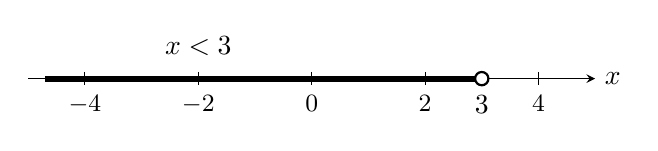
\begin{tikzpicture}[x=.72cm,y=.72cm,>=stealth]
\draw[->] (-5,0)--(5,0) node[right] {$x$};
\foreach \x in {-4,-2,0,2,4}{\draw (\x,.12)--(\x,-.12) node[below] {\small $\x$};}
\draw (3,.12)--(3,-.12) node[below] {$3$};
\draw[line width=2.2pt] (-4.7,0)--(3,0);
\draw[fill=white,thick] (3,0) circle (2.4pt);
\node[above] at (-2,0.23) {$x<3$};
\end{tikzpicture}
\end{center}
\poznamka{Geometricky: násobení číslem $-1$ je zrcadlení číselné osy podle nuly. Čísla vlevo se dostanou vpravo a obráceně. Na původní ose $x$ proto vždy zapisujeme stejný výsledný interval.}

\blok{Řešené příklady: od jednoduchého ke složitějšímu}
\begin{prikladReseniBox}[title={Příklad 2}]
Vyřešte $3x-5>7$.
\tcblower
\[
\begin{aligned}
3x-5&>7 \\
 3x&>12 \\
 x&>4
\end{aligned}
\]

Číslo $4$ není řešením.
\[
\begin{aligned}
K &= (4;+\infty)
\end{aligned}
\]
\end{prikladReseniBox}
\begin{prikladReseniBox}[title={Příklad 3}]
Vyřešte $-2(x-3)\le4x+6$.
\tcblower
\[
\begin{aligned}
-2x+6&\le4x+6 \\
 -6x&\le0 \\
 x&\ge0
\end{aligned}
\]

Při dělení $-6$ se nerovnost obrací.
\[
\begin{aligned}
K &= \langle0;+\infty)
\end{aligned}
\]
\end{prikladReseniBox}
\poznamka{Po každé úpravě záporným číslem nahlas požaduj zdůvodnění obrácení znaménka.}
\blok{Samostatné procvičování}
\begin{zadaniReseniBox}[title={Samostatná práce 1}]
$x+3<1$.
\tcblower
\[
\begin{aligned}
x&<1-3 \\
 x&<-2 \\[2mm]
K &= (-\infty;-2)
\end{aligned}
\]
\end{zadaniReseniBox}
\begin{zadaniReseniBox}[title={Samostatná práce 2}]
$5-3x\ge2$.
\tcblower
\[
\begin{aligned}
-3x&\ge-3 \\
 x&\le1 \\[2mm]
K &= (-\infty;1\rangle
\end{aligned}
\]
\end{zadaniReseniBox}
\begin{zadaniReseniBox}[title={Samostatná práce 3}]
$4(x-1)>2x+6$.
\tcblower
\[
\begin{aligned}
4x-4&>2x+6 \\
 2x&>10 \\
 x&>5 \\[2mm]
K &= (5;+\infty)
\end{aligned}
\]
\end{zadaniReseniBox}
\blok{Volitelná rezerva}
\begin{zadaniReseniBox}[title={Samostatná práce 4}]
Proč není bezpečné vynásobit $x>1$ neznámým výrazem $x-3$?
\tcblower
\[
\begin{aligned}
x&>1\quad\text{a}\quad x-3\lessgtr0
\end{aligned}
\]

Činitel $x-3$ mění znaménko v $x=3$. Bez rozboru nelze stanovit směr nové nerovnosti.
\end{zadaniReseniBox}
\begin{zadaniReseniBox}[title={Rozšíření 1}]
Vyřešte $(x-1)^2-(x+1)^2<8$.
\tcblower
\[
\begin{aligned}
(x^2-2x+1)-(x^2+2x+1)&<8,\\
-4x&<8,\\
x&>-2.
\end{aligned}
\]
Všimněte si, že členy $x^2$ se vyrušily: výsledkem je lineární nerovnice.
\[
\begin{aligned}
K &= (-2;+\infty)
\end{aligned}
\]
\end{zadaniReseniBox}
\blok{Domácí úkol}
\begin{zadaniReseniBox}[title={Domácí úkol}]
\begin{enumerate}[label=\alph*)]
\item
$7-2x<1$.
\item
$-(x+4)\ge3$.
\item
$\frac{x-1}{2}\le3$.
\item
$3x-5<7$.
\item
$4-3(2x-1)\ge1$.
\item
$-2(x-3)>4x+6$.
\end{enumerate}
\tcblower
\begin{enumerate}[label=\alph*)]
\item
\[
\begin{aligned}
-2x&<-6 \\
 x&>3 \\[2mm]
K &= (3;+\infty)
\end{aligned}
\]
\item
\[
\begin{aligned}
-x-4&\ge3 \\
 -x&\ge7 \\
 x&\le-7 \\[2mm]
K &= (-\infty;-7\rangle
\end{aligned}
\]
\item
\[
\begin{aligned}
x-1&\le6 \\
 x&\le7 \\[2mm]
K &= (-\infty;7\rangle
\end{aligned}
\]
\item
\[
\begin{aligned}
3x&<12\\x&<4 \\[2mm]
K &= (-\infty;4)
\end{aligned}
\]
\item
\[
\begin{aligned}
7-6x&\ge1\\-6x&\ge-6\\x&\le1 \\[2mm]
K &= (-\infty;1\rangle
\end{aligned}
\]
\item
\[
\begin{aligned}
-2x+6&>4x+6\\-6x&>0\\x&<0 \\[2mm]
K &= (-\infty;0)
\end{aligned}
\]
\end{enumerate}
\end{zadaniReseniBox}
\poznamka{Orientační časové rozvržení: 5 + 12 + 12 + 10 + 6 = 45 min. Přednost má pochopení jádra; rezerva není součástí časového součtu. Domácí úlohy jsou určeny na samostatnou práci, řešení zůstávají učiteli.}
\end{document}
